\documentclass[sigconf,anonymous,review]{acmart}

\AtBeginDocument{\providecommand\BibTeX{{Bib\TeX}}}
\setcopyright{none}
\settopmatter{printacmref=false, printccs=true}
\renewcommand\footnotetextcopyrightpermission[1]{}

\usepackage{tabularx}
\usepackage{array}
\usepackage{balance}
\usepackage{xspace}
\emergencystretch=2em

\newcommand{\appfp}{\textsc{App177}\xspace}
\newcommand{\browserfp}{\textsc{Browser67}\xspace}
\newcommand{\pairedfp}{\textsc{paired244}\xspace}

\begin{document}

\title{HybridGuard: Provenance-Aware Cross-Layer Fingerprint Consistency for Android Web Environments}

\author{Anonymous Author(s)}
\affiliation{%
  \institution{Anonymous Institution}
  \country{Anonymous}}
\email{anonymous@example.com}
\renewcommand{\shortauthors}{Anonymous Author(s)}
\acmConference[Working Draft]{HybridGuard Working Draft}{September 2026}{Anonymous}
\acmYear{2026}
\copyrightyear{2026}
\acmDOI{}
\acmISBN{}

\begin{abstract}
Android hybrid applications expose the same execution environment through several partially overlapping surfaces: Android Native APIs, the WebView host, JavaScript running inside the app, and, in some workflows, an independent system browser. An adversary can manipulate individual browser-facing attributes, but preserving a coherent representation across these surfaces requires coordinating APIs, containers, versions, and host-controlled state. We present the design and current controlled evidence for \emph{HybridGuard}, a provenance-aware framework that collects fixed-contract multi-layer fingerprints, records per-field availability states, derives explicit cross-layer evidence, and evaluates source-separated semantic relations without exposing attack labels or collection shortcuts to the decision path. The current controlled evaluation deliberately uses \appfp---84 Native, 26 WebView-host, and 67 in-app Web signals---because sufficiently complete external-browser attack pairs are not yet available. Under a verified two-state protocol, 229 normal observations and 69 qualified \emph{baseline $\rightarrow$ attack-active} pairs are analyzed. On this frozen cohort, nine project-derived relations grounded in official field semantics produce 51 baseline-no-alert to active-alert transitions, while ten independently maintained device-mined predicates produce 33. We report these values as controlled relation-coverage observations, not as attack recall or production risk-based-authentication performance. Separately, HybridGuard implements an independent \browserfp collector and provenance-complete \pairedfp data path, including honest App-only retention when browser capture is incomplete. Evaluating the incremental detection value and benign variability introduced by \browserfp is left to a future, sufficiently complete paired-data study.
\end{abstract}

\begin{CCSXML}
<ccs2012>
 <concept>
  <concept_id>10002978.10003022.10003028</concept_id>
  <concept_desc>Security and privacy~Web application security</concept_desc>
  <concept_significance>500</concept_significance>
 </concept>
 <concept>
  <concept_id>10002978.10003022.10003023</concept_id>
  <concept_desc>Security and privacy~Software security engineering</concept_desc>
  <concept_significance>300</concept_significance>
 </concept>
 <concept>
  <concept_id>10002978.10002997</concept_id>
  <concept_desc>Security and privacy~Intrusion/anomaly detection and malware mitigation</concept_desc>
  <concept_significance>300</concept_significance>
 </concept>
</ccs2012>
\end{CCSXML}

\ccsdesc[500]{Security and privacy~Web application security}
\ccsdesc[300]{Security and privacy~Software security engineering}
\ccsdesc[300]{Security and privacy~Intrusion/anomaly detection and malware mitigation}

\keywords{browser fingerprinting, Android WebView, hybrid applications, cross-layer consistency, provenance, controlled manipulation, risk-based authentication}

\maketitle

\section{Introduction}
\label{sec:introduction}

Device and browser fingerprints occupy an uneasy position in Web security. They can provide a passive signal for associating a request with a previously observed environment, augmenting passwords or informing risk-based authentication (RBA) decisions~\cite{alaca2016device,papaioannou2023survey}. At the same time, mobile fingerprints may be insufficiently distinctive or stable to serve as a trusted-device factor on their own~\cite{spooren2015harmful}, and the same attributes can be used for unwanted tracking~\cite{laperdrix2020browser,w3c2025fingerprinting}. A security system therefore cannot treat a long feature vector, or even a highly distinctive value, as an integrity proof. It must reason about where each observation came from, whether it was available under the current platform conditions, which relationships are expected to hold, and which deviations admit benign explanations.

The adversarial setting makes this requirement more acute. Browser-facing attributes can be altered through injected scripts, browser configuration, debugging interfaces, automation frameworks, or purpose-built evasion services. Gummy Browsers demonstrates that a targeted adversary can capture a victim fingerprint and orchestrate another browser to imitate it~\cite{liu2022gummy}. Large-scale measurements of commercial traffic likewise show that adversarial and benign fingerprints form a meaningful problem for deployed Web defenses~\cite{wu2023manyfaces}. Yet manipulating isolated attributes is not equivalent to producing a coherent environment. FP-Scanner showed that anti-fingerprinting countermeasures often introduce contradictory combinations of browser attributes~\cite{vastel2018fpscanner}; more recently, FP-Inconsistent found spatial and temporal inconsistencies in evasive bot traffic and learned rules that expose part of this manipulation~\cite{venugopalan2025fpinconsistent}. BrowserFM further demonstrates that browser attributes can be linked systematically to the configurations and environments that generate them~\cite{huyghe2025browserfm}. These studies establish consistency as an important signal, but they primarily reason \emph{within} a browser fingerprint or between a browser and its generating configuration.

Android hybrid applications expose a broader boundary. The host application can observe Native build, hardware, display, memory, sensor, installation, and debugging state. The WebView host contributes provider, package, JavaScript-bridge, user-agent, and security-configuration information. JavaScript inside the embedded page sees a browser-like runtime containing navigator, screen, viewport, Canvas, WebGL, timezone, resource, and automation-facing properties. These surfaces are technically distinct but operationally coupled. Android applications can customize WebView behavior and create explicit Java--JavaScript channels; recent large-scale studies show that these channels are widely used to connect native identifiers, Web APIs, tracking code, and network destinations~\cite{weerasekara2025tracking,datta2026crossboundary}. Earlier systems such as BridgeTaint and iWanDroid demonstrate that security-relevant evidence must often be tracked across the Java--JavaScript boundary rather than analyzed on one side alone~\cite{bai2019bridgetaint,tiwari2023demand}.

This paper asks a different question from information-flow or tracking measurement: \emph{can the multiple observations produced during one controlled Android hybrid-app session be treated as provenance-bound integrity evidence, and which explicit relationships change when part of the environment is manipulated?} A Native Android 13 observation paired with a desktop Windows user agent is not merely an unusual browser string; it contradicts the host surface that produced the Web runtime. A WebView provider version and a runtime Chromium version may be comparable only at a coarse major-version level. A physical-resolution relation requires orientation, insets, viewport, and density tolerance. A missing Browser capture is not a vector of zeroes, and an unparseable user agent is not evidence that two versions match. These distinctions motivate HybridGuard.

HybridGuard is a research framework for fixed-contract collection, provenance-aware pairing, deterministic evidence extraction, source-separated relation execution, and auditable reporting. Its current in-app collection unit, \appfp, contains 84 Android Native signals, 26 WebView-host signals, and 67 in-app Web-runtime signals. Each field is accompanied by a state such as observed, unsupported, permission-denied, runtime-error, timeout, or not-applicable. Accepted payloads are bound to collection receipts, batches, release identifiers, payload hashes, and quality-control records. Deterministic extractors convert raw fields into an evidence bundle containing parsed facts, cross-layer comparisons, applicability conditions, and explicit unassessed states. Relations derived from official Android/Chrome field semantics are maintained separately from empirically mined predicates; official documents ground what a field means, but the resulting risk relation remains a project inference.

The current controlled experiment uses \appfp only. This is a deliberate evidence boundary rather than an assertion that the external browser is unimportant: the repository contains an independent \browserfp probe and a provenance-complete \pairedfp path, but complete external-browser observations are currently too sparse for a defensible attack-effect evaluation. We therefore evaluate verified two-state \emph{baseline $\rightarrow$ attack-active} pairs over the three in-app layers, report exactly which fields changed, which relations became violated, and which configurations remain uncovered. Once sufficiently complete paired data are collected, the same protocol will be rerun to compare \appfp-only, \browserfp-only where meaningful, and joint \pairedfp variants.

On the current frozen cohort, 229 normal observations and 69 qualified controlled pairs are available. Nine executable semantic relations grounded in official field definitions yield 51 baseline-no-alert to active-alert transitions; ten independently maintained device-mined predicates yield 33. Thirty-three pairs trigger both sources, eighteen trigger only the official-derived relation set, and eighteen trigger neither. The uncovered pairs include manipulations restricted to WebDriver, resource values, languages, plugins/MIME types, timezone, and screen metrics. These values characterize the behavior of frozen rules on frozen controlled configurations. They are \emph{not} an estimate of population-level recall, benign false-positive rate, unknown-attack generalization, or production RBA effectiveness.

Taken together, this draft makes five connected contributions. First, it introduces a provenance-aware multi-surface data model that combines fixed App and external-browser contracts with per-field state semantics, receipt/batch/hash binding, provenance-complete pairing, and honest App-only retention when browser capture is incomplete. The collection and pairing path is already implemented, although large-scale paired attack data remain future work. Second, it converts \appfp payloads into deterministic Native--WebView--Web evidence whose relations explicitly encode applicability, tolerance, counterexamples, and not-assessed outcomes rather than treating missing data as normal or directly concatenating all raw fields. Third, it separates project-derived semantic relations grounded in official field definitions from device-mined predicates, executes the two sources independently, and retains the field-level evidence that supports each decision. Fourth, it evaluates these frozen relation sets on verified baseline-to-active pairs supplied by the controlled-manipulation workstream and reports both observed alert transitions and concrete coverage gaps without relabeling the counts as attack recall. Finally, it establishes an implemented \browserfp and \pairedfp data path while reserving any claim about the incremental detection value of the external-browser surface for a later complete-data ablation.

The remainder of this draft first positions HybridGuard relative to device-fingerprint authentication, browser inconsistency detection, and Android WebView analysis (Section~\ref{sec:background-related}). It then defines the observation surfaces and threat model (Section~\ref{sec:problem}), presents the system and evidence pipeline (Sections~\ref{sec:system} and~\ref{sec:evidence}), specifies the two-state experimental methodology (Section~\ref{sec:methodology}), reports the current \appfp results (Section~\ref{sec:current-results}), and separates historical preliminary evidence from the future \browserfp study (Sections~\ref{sec:historical} and~\ref{sec:browser-future}).

\section{Background and Related Work}
\label{sec:background-related}

\subsection{Device Fingerprints as Authentication Context}

Browser fingerprinting combines software, hardware, and runtime attributes exposed through HTTP headers and Web APIs into a probabilistic representation of a client environment~\cite{laperdrix2020browser,eckersley2010unique}. The same mechanism supports several distinct applications: stateless tracking, fraud analysis, bot detection, account protection, and adaptive authentication. These applications must not be conflated. A field that is useful for population-level linkability may be unstable across software updates; an attribute that is inexpensive to collect may be inexpensive to spoof; and a fingerprint that distinguishes desktop configurations may collapse many mobile devices into similar profiles.

Alaca and van Oorschot analyze device fingerprinting specifically as an auxiliary Web-authentication factor. Rather than ranking methods by uniqueness alone, they classify 29 approaches and compare properties including stability, repeatability, passiveness, resource cost, spoofing difficulty, and distinguishability~\cite{alaca2016device}. This framing is directly relevant to HybridGuard: the goal is not to maximize the entropy of a single identifier but to collect low-friction context whose limitations are explicit. Spooren et al. provide an important counterweight, finding that mobile device fingerprints can exhibit substantial similarity even across models and brands, which weakens their reliability as a standalone trusted-device signal for RBA~\cite{spooren2015harmful}. Empirical work on deployed RBA also shows that real services combine multiple context factors and apply different thresholds rather than treating a fingerprint as a cryptographic identity~\cite{wiefling2019really}.

HybridGuard follows the conservative implication of this literature. It does not claim that \appfp identifies a physical device uniquely or that a relation alert proves account fraud. Instead, it treats multiple surfaces from the same controlled session as evidence about environment coherence. The downstream consumer may be an RBA policy, but the evaluated task in this paper is device-environment manipulation and cross-layer relation violation.

\subsection{Browser Fingerprint Spoofing and Adversarial Use}

The security use of fingerprints creates an incentive to manipulate them. Large commercial measurements have characterized both benign and adversarial browser fingerprints observed by production-facing services~\cite{wu2023manyfaces}. Gummy Browsers studies a targeted form of the threat: an attacker first collects a victim's browser fingerprint and then changes a separate browser through script injection, script modification, browser settings, or debugging tools so that fingerprint-linking systems associate the attacker with the victim~\cite{liu2022gummy}. The work demonstrates that browser-exposed surfaces are not immutable and motivates controlled manipulations of User-Agent, platform, WebGL, resources, and automation-facing properties.

HybridGuard adopts this adversarial premise but evaluates a narrower and more auditable question. The controlled-manipulation workstream records the exact tool, runner, version, configuration, and affected field paths, and provides verified baseline-to-active pairs. The main analysis does not infer an attack label from a tool name, a process return code, or the existence of a WebDriver marker. It first verifies that a catalogued field actually changed and only then asks whether a frozen relation becomes violated. This distinction is necessary because automation and debugging interfaces also have legitimate testing uses, and because a successfully executed intervention may not affect the fields observed by the current collector.

\subsection{Fingerprint Inconsistency and Configuration Relations}

The closest line of prior work detects contradictions inside browser fingerprints. FP-Scanner examines anti-fingerprinting countermeasures and shows that partial attribute modification can create combinations that do not naturally correspond to one browser or operating-system configuration~\cite{vastel2018fpscanner}. The scanner can use such contradictions to detect the presence of countermeasures and, for some attributes, infer the original environment. FP-Inconsistent revisits the idea in evasive bot traffic at larger scale. Its honey-site study shows that commercial bot services alter different fingerprint attributes to bypass anti-bot services, yet leave spatial inconsistencies within one fingerprint and temporal inconsistencies across observations~\cite{venugopalan2025fpinconsistent}. The paper learns rules from these inconsistencies and demonstrates that they expose part of the measured evasion.

BrowserFM attacks a related representation problem. It generates browser fingerprints under many Chromium versions, hardware environments, and configuration parameters, then links fingerprints, configurations, and environments through feature models and per-observation identifiers~\cite{huyghe2025browserfm}. The result supports queries such as which attributes respond to a particular switch, how headless and headful configurations differ, and which reduced attribute sets retain configuration information. Earlier cross-browser fingerprinting likewise demonstrates that OS- and hardware-level properties can remain observable across browser implementations~\cite{cao2017crossbrowser}, while GPU work shows that Web rendering can reveal low-level hardware variation~\cite{laor2022drawnapart}.

HybridGuard shares the premise that relationships carry information beyond isolated values. Its analysis boundary, however, is different. FP-Scanner and FP-Inconsistent primarily inspect browser-internal relations; BrowserFM studies configuration generation; cross-browser fingerprinting studies linkability. HybridGuard binds observations from Android Native APIs, the WebView host, and the in-app Web runtime to one collection provenance and evaluates explicit cross-layer semantics under controlled intervention. It also treats unavailable, unparseable, and not-applicable fields as distinct from matching values. Consequently, the closest browser systems are conceptual neighbors rather than drop-in baselines.

\subsection{Android WebView and Cross-Boundary Observability}

Android hybrid applications combine at least two programming and security domains. Native code controls the application process, permissions, package state, and WebView configuration; JavaScript executes under browser-origin and Web API semantics. Large-scale work on Android--Web hybridization documents the prevalence and architectural complexity of these combinations~\cite{tiwari2020hybridization}. Android's own documentation emphasizes that JavaScript bridges and WebView settings alter the boundary between untrusted Web content and application capabilities~\cite{android2026nativebridges,android2026webview,android2026websettings}.

Several systems analyze this boundary as an information-flow problem. BridgeTaint propagates taint information bi-directionally through JavaScript bridges and maps labels across the language boundary to identify privacy leaks and code injection paths~\cite{bai2019bridgetaint}. iWanDroid takes a demand-driven approach, selectively summarizing Native code according to how JavaScript consumes exposed functionality, so that information-flow violations can be followed in both directions~\cite{tiwari2023demand}. These works establish that a WebView cannot be analyzed faithfully by treating Native and JavaScript code as independent programs.

Recent measurement studies examine how the same boundary is used in deployed applications. Tracking Without Borders combines static and dynamic analysis over 13,045 Google Play applications and reports widespread WebView customization, browser fingerprinting, identifier bridging, cookie syncing, and access to permission-protected resources~\cite{weerasekara2025tracking}. Cross-Boundary Mobile Tracking introduces WebViewTracer, combining Frida-observed Java method calls with VisibleV8 JavaScript execution traces. On 10,000 applications, it identifies sensitive information injected from Java into WebViews and subsequently sent through Web APIs, while also observing fingerprinting behavior inside WebView scripts~\cite{datta2026crossboundary}. These results show that the host and Web runtime form an operationally coupled system even though their security contexts differ.

HybridGuard is adjacent to, but distinct from, this work. It does not attempt full source-to-sink taint tracking, SDK attribution, or detection of privacy exfiltration. Its inputs are fixed runtime observations collected by a purpose-built app, and its output is a versioned set of environment facts and relation states. A JavaScript bridge is therefore treated as host-topology evidence, not as proof of a leak; a WebView user-agent override may be legitimate and is encoded as a tolerance or not-assessed case rather than a universal alert.

\subsection{Detecting Fingerprinting Scripts versus Validating Environment Evidence}

Another body of work detects whether a Web page or application performs fingerprinting. FP-Fed trains privacy-preserving detectors for fingerprinting scripts~\cite{annamalai2024fpfed}; FP-tracer analyzes API-level information flow and entropy to identify fingerprinting behavior~\cite{boussaha2024fptracer}; Android-focused work detects fingerprinting activity inside application code~\cite{heid2024androidfp}. These systems answer a different question from HybridGuard. In HybridGuard, collection is intentional and declared. The question is whether the resulting Native, host, and Web observations form a provenance-complete and semantically compatible environment under the current experimental facts.

This task distinction changes both labels and evaluation. A fingerprinting-script detector may use script behavior as a positive label. HybridGuard must not: a page can legitimately read a fingerprint field, an automation interface can be used for testing, and a field may differ across containers without implying maliciousness. The project therefore separates collection metadata, verified intervention facts, model-visible evidence, and final relation status.

\subsection{Positioning Summary}

Table~\ref{tab:positioning} summarizes the closest task boundaries. The novelty claim in this draft is deliberately compositional: the contribution is the combination of Android multi-layer collection, per-field states, provenance-complete data units, explicit relation applicability, source-separated rules, and controlled two-state evaluation. The draft does not claim to be the first use of fingerprint consistency, the first cross-language WebView analysis, or a complete RBA system.

\begin{table*}[t]
\caption{Positioning against the closest lines of work. ``Controlled pairs'' means that the primary evaluation unit explicitly binds a baseline and a verified active intervention.}
\label{tab:positioning}
\small
\begin{tabularx}{\textwidth}{@{}p{2.8cm}p{2.5cm}p{2.4cm}p{2.2cm}X@{}}
\toprule
Line of work & Main observation boundary & Primary task & Controlled pairs & Difference from HybridGuard \\
\midrule
FP-Scanner / FP-Inconsistent & Browser attributes & Detect altered or evasive fingerprints & Not HybridGuard-style App pairs & Browser-internal spatial/temporal consistency; no Android Native--WebView provenance contract \\
Gummy Browsers & Victim and attacker browsers & Targeted fingerprint impersonation & Attack experiments, but different unit & Demonstrates spoofability; HybridGuard evaluates environment contradictions rather than identity linkage \\
BrowserFM & Browser, configuration, system & Structured configuration analysis & Configuration enumeration & Preserves generating configuration; does not evaluate Android cross-layer manipulation \\
BridgeTaint / iWanDroid & Java--JavaScript flows & Leakage, injection, information-flow violations & No & Code/data-flow analysis rather than runtime environment consistency \\
Tracking Without Borders / WebViewTracer & App, SDK, WebView, JavaScript, network & Privacy tracking and cross-context diffusion & No & Large-scale behavior measurement rather than fixed-contract evidence comparison \\
HybridGuard (current) & Android Native, WebView host, in-app Web & Provenance-aware relation violation & Yes: baseline $\rightarrow$ active & Reports field effects, applicability, alerts, and uncovered controlled configurations \\
HybridGuard (future) & Current layers plus external browser & Incremental Browser67 value & Planned & Requires sufficiently complete paired244 attack and benign data \\
\bottomrule
\end{tabularx}
\end{table*}

\section{Problem Formulation and Threat Model}
\label{sec:problem}

This section formalizes the evidence unit, adversary, and evaluation task used throughout the paper. The current empirical study is intentionally restricted to \appfp observations collected under a verified two-state protocol. The independent external-browser surface is already part of the data architecture, but its attack-effect contribution is treated as a separate research question because the present collection does not yet contain enough complete \browserfp pairs for a defensible comparison.

\subsection{Observation Surfaces}

HybridGuard models a mobile hybrid-app session as a set of logically distinct observation surfaces rather than referring to them collectively as ``three endpoints.'' The distinction matters because each surface is controlled by a different software layer, exposes different APIs, and admits different benign sources of variation.

The first surface is \emph{Android Native}. It contains signals obtained from Android framework and system APIs, including release and build identity, hardware family, physical display properties, memory, sensor availability, battery context, package and installation state, and debugging context. These observations describe the host application and operating environment from the perspective of Native code. The second surface is the \emph{WebView host}. It records properties controlled by the embedded-browser container and the application that instantiates it, such as WebView provider and version, the default user agent, JavaScript-bridge topology, package and installation context, WebView debugging, cleartext policy, and application configuration. Although the WebView host executes in the same application process as Native code, its security and versioning semantics differ from those of the Android framework.

The third surface is the \emph{in-app Web runtime}. It is collected by JavaScript executing inside the FeatureApp WebView and includes browser-visible navigator and platform values, runtime user agent, logical screen and viewport geometry, device-pixel ratio, timezone, Canvas and WebGL outputs, language and plugin/MIME surfaces, resource indicators, and automation-facing attributes. This surface resembles a conventional browser fingerprint, but it is produced inside an application-controlled WebView rather than a standalone browser. The fourth surface is the \emph{external browser}. The same Web probe is launched in an independent system browser and produces \browserfp. It is deliberately modeled as a separate context: similarly named APIs need not return identical values because the WebView and the system browser may use different versions, processes, permissions, storage state, viewport settings, network paths, or customization policies.

The current in-app observation can be written as $x_{\mathrm{app}}=(x_N,x_H,x_W)$, where the three components denote the Native, WebView-host, and in-app Web surfaces. Their frozen dimensions are 84, 26, and 67 signals, respectively. A completed external-browser observation $x_B$ contributes another 67 signals. The derived paired observation $x_{\mathrm{pair}}=(x_{\mathrm{app}},x_B)$ enters the \pairedfp view only when both payloads and their receipts, hashes, collection batches, and pair-provenance records satisfy the frozen contract. When $x_B$ is unavailable, the valid App observation remains an explicit App-only record rather than being padded with artificial Browser values.

\subsection{Field Values, Availability States, and Control Metadata}

For every field $f$, HybridGuard stores a value $v_f$ separately from an availability state $s_f$. The state vocabulary distinguishes an observed value from an unsupported API, permission denial, runtime error, timeout, and a field or relation that is not applicable in the current context. Relation evaluation consumes $(v_f,s_f)$ rather than a value alone, so a parser default or an empty serialization cannot silently convert unavailable evidence into a legitimate zero, false value, or empty string.

Collection and experimental metadata are maintained on a separate control plane. Session identifiers, receipts, batch identifiers, canonical payload hashes, pair identifiers, provider labels, intervention tools, experiment phases, stable-group keys, data splits, and verified labels are used for admission, grouping, and audit, but they are excluded from model-visible evidence. This separation prevents unavailable numeric values from being mistaken for zeroes, prevents a failed Browser launch from becoming an apparently complete 244-field sample, and prevents source names or experiment roles from becoming easier decision shortcuts than the intended environment relationships.

\subsection{Controlled Manipulation Adversary}

The evaluated adversary applies a documented intervention after a baseline collection. Depending on the configuration, it can use Chrome DevTools Protocol controls, Playwright, Puppeteer, Stealth plugins, browser emulation, JavaScript interception, or related runtime mechanisms to modify the WebView or in-app Web surface. The controlled configurations target individual or combined properties such as User-Agent, platform, WebDriver, languages, plugin and MIME surfaces, WebGL vendor and renderer strings, resource values, timezone, and screen or viewport metrics.

This adversary model is intentionally bounded. It does not assume compromise of the Android kernel, successful forgery of hardware-backed attestation, or arbitrary coherent rewriting of every collector output. At the same time, HybridGuard does not equate successful tool execution with an observable attack effect. A comparison enters the current analysis only when independent evidence supports the intervention and direct payload comparison confirms at least one change to a catalogued field. This requirement matters because automation and debugging interfaces have legitimate testing uses, some interventions affect fields outside the collector, and a tool may execute without producing the intended mutation under a particular Android or WebView version.

\subsection{Two-State Evaluation Unit}

Following the advisor's requirement, the paper uses exactly two states, $x^{(b)}\rightarrow x^{(a)}$, where $x^{(b)}$ is the baseline observation and $x^{(a)}$ is collected while the intervention is active. Historical \texttt{clean\_post} records are not used as eligibility conditions, denominators, or evidence for the conclusions in this manuscript. A qualified pair binds the baseline and active observations to the same scenario group and compatible release and schema context while retaining the exact intervention configuration on the control plane.

Each executable relation combines an applicability condition with a comparison and returns one of four states. A \emph{consistent} or \emph{inconsistent} result records the outcome of an applicable comparison, while a \emph{context} result preserves relevant evidence that is not itself a strong alert. The evaluator returns \emph{not assessed} when required evidence is unavailable, unparseable, or outside the declared scope. The principal current observation is a transition from a baseline with no strong relation alert to an active observation with such an alert. That transition describes one frozen relation set on one verified controlled pair; it is not, by itself, a population-level detection metric.

\subsection{Task Boundary and Non-Goals}

The current task is to determine which explicit relationships among the Native, WebView-host, and in-app Web surfaces are violated by verified controlled manipulations, which relations cannot be evaluated, and which confirmed field changes remain outside the frozen relation set. It is therefore distinct from identifying a physical device or tracking a user across sites, proving that an account action is fraudulent, detecting every script that performs fingerprinting, reconstructing complete WebView information flows, classifying malware, or providing cryptographic remote attestation. The study also does not assume that any difference between the in-app runtime and the external browser is malicious, and it does not evaluate the end-to-end effectiveness or user cost of a production RBA policy.

RBA remains the motivating downstream setting. A well-validated environment-integrity signal could inform step-up authentication, restricted access, or manual review. Demonstrating that policy benefit would require account-level ground truth, representative benign and malicious traffic, calibrated thresholds, and user-impact measurements that are not available in the present controlled dataset.

\subsection{Research Questions}

The study is organized around four research questions. \emph{RQ1} asks whether fixed \appfp and \browserfp observations can be governed through explicit field states, release locks, receipts, hashes, and provenance-complete pairing while retaining valid App observations when Browser collection fails. \emph{RQ2} asks which cross-layer \appfp relations change under verified baseline-to-active manipulations and which configurations remain uncovered or unassessed. \emph{RQ3} asks what incremental evidence and benign variability the independently collected \browserfp surface introduces beyond \appfp once sufficiently complete paired data are available. Finally, \emph{RQ4} asks how official-derived relations, device-mined predicates, raw-feature baselines, explicit consistency features, and knowledge-grounded reasoning compare when evaluation is separated by stable device or profile and by controlled scenario. The current results answer RQ2 at a mechanism level, the implemented data path partially addresses RQ1, and RQ3--RQ4 require the future grouped study specified later in the paper.

\section{HybridGuard Design}
\label{sec:system}

\begin{figure*}[t]
  \centering
  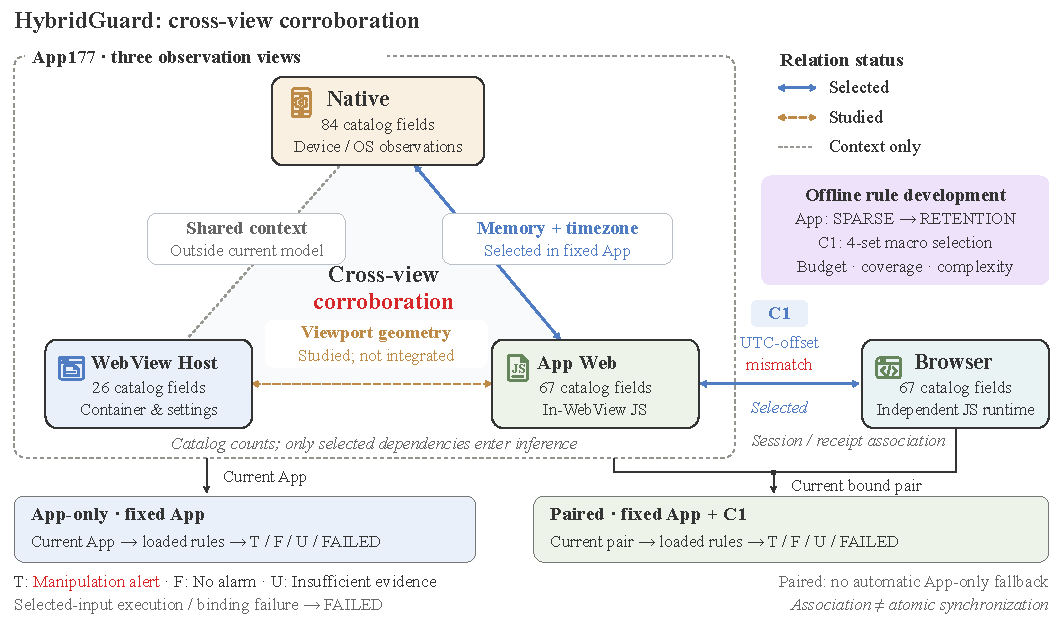
\includegraphics[width=\textwidth]{figures/HybridGuard_overview_triangle.pdf}
  \caption{HybridGuard as a triangle of complementary observation views. Native, WebView Host, and App Web provide device/system, container/settings, and webpage-runtime observations. Solid blue edges denote relations selected in the retained models: Native--App Web memory and timezone relations, and the App Web--independent Browser numeric UTC-offset condition C1. The dashed ochre edge denotes separately studied Host geometry that is not integrated; the arrowless dotted gray edge denotes only shared Native--Host context outside the current App rule pool. Arrowed comparison edges identify the views being compared, not bidirectional rule execution or trusted ground truth. The App detector combines within-view rules with selected cross-view relations. Offline development applies App SPARSE selection and RETENTION, followed by constrained macro-detection selection over four cross-endpoint sets. Separate App-only and paired interfaces load fixed models and read only current inputs. T denotes a manipulation alert, F no alarm, and U insufficient evidence; execution or binding failures in selected inputs take precedence as FAILED. Paired inference has no automatic App-only fallback. Field counts describe catalogs, binding IDs are not detection features, and association does not imply atomic synchronization.}
  \Description{Native, WebView Host, and App Web form a triangle. Selected memory and timezone comparisons use a solid blue edge; separately studied geometry uses a dashed ochre edge. The arrowless dotted gray edge denotes shared context only. The independent Browser is outside the triangle and connected to App Web by C1. Offline development is separate from the two current-input interfaces.}
  \label{fig:hybridguard-overview}
\end{figure*}


Figure~\ref{fig:hybridguard-overview} provides an overview of the observation views and their relationships.

HybridGuard is organized as an auditable chain from collection to relation evidence rather than as a monolithic classifier. The current repository implements the multi-layer collector, backend provenance records, snapshot construction, App evidence extraction, deterministic relation execution, verification, and trace generation. Browser-aware decision logic, a large-scale public benchmark, and calibrated production decisions remain later stages. The architecture nevertheless represents these later stages explicitly so that the current data products can evolve without changing their meaning.

\subsection{Design Principles}

The design begins with a fixed-contract view of fingerprint collection. The active release publishes a versioned field catalog and a corresponding state entry for each signal. Adding, deleting, renaming, or changing the type of a signal requires an explicit schema revision; an older payload is not padded with defaults and relabeled as current. This choice makes the field count meaningful and allows every result to be tied to the exact collector and catalog that produced it.

Fusion is permitted only after provenance has been established. App and external-browser payloads remain independent canonical records in the backend, each with its own receipt and content hash. The system derives a joint view only when the associated batch, receipts, hashes, and pair events close successfully. This ``provenance before fusion'' rule prevents a convenient row-level join from being mistaken for evidence that two observations actually came from the intended collection episode.

Missingness is treated as part of the evidence model rather than as a preprocessing inconvenience. Unsupported APIs, denied permissions, timeouts, runtime errors, and not-applicable relations have different meanings, and the system preserves those meanings through the snapshot and evidence layers. In particular, the absence of an external-browser observation never becomes 67 zero-valued fields. A valid App payload remains usable as App-only evidence, while the missing Browser side is represented in the control plane with an explicit terminal status.

The reasoning path is also deliberately staged. Parsing, normalization, field-family classification, relation applicability, and direct comparisons are computed deterministically before any optional model is involved. Historical LLM prototypes may interpret or summarize this evidence, but they do not define whether an Android version parsed successfully or whether a WebView-provider major version equals a runtime Chromium major version. Finally, labels and shortcut-prone metadata stay outside the runtime. Tool names, provider identities, stable groups, pair roles, splits, and verified facts are used to construct and audit an experiment, not to trigger the relation evaluator.

\subsection{Collection Architecture}

The FeatureApp coordinates the three in-app surfaces. Native code first records Android and device state and captures WebView-host properties. It then loads the versioned Web probe inside the application WebView, receives the JavaScript-visible runtime measurements, and packages the three layers into an \appfp payload together with a collection manifest and per-field states. The backend stores a canonical raw representation, computes or verifies the payload hash, issues a receipt, and associates the record with the current process-lifecycle collection batch. Analysis projections may be generated for convenience, but the canonical raw payload and its receipt remain the authoritative source.

The external-browser path begins only after the App-side collection has enough provenance to request a companion observation. The backend creates a short-lived pairing context, and the application launches the system browser to the independent Web probe. A completed \browserfp upload receives its own raw record and is linked to the initiating App session through pair events and a completed pair-provenance object. The pair record identifies the two canonical payloads; it does not replace them with a new untraceable upload.

The two uploads are asynchronous and may fail independently. This property is important in mobile testing, where browser launch restrictions, foreground transitions, provider behavior, timeouts, and platform support can prevent the companion probe from completing even after a valid App payload has been accepted. HybridGuard therefore produces four logically different products. A provenance-complete App and Browser pair becomes a derived \pairedfp record. A valid App whose Browser attempt is incomplete or unsupported remains in the App-only 177 view. Records that violate release, schema, receipt, batch, hash, or provenance constraints enter quarantine with an explicit reason. Session identifiers, receipts, pair identifiers, batch metadata, and selection decisions are retained in a sample index and audit files rather than mixed into the signal vector.

This separation lets downstream consumers choose an evidence unit honestly. An App-only analysis operates on 177 observed signals and their states. A paired analysis requires the completed 244-field view. Neither path silently changes dimensionality based on convenience, and the failure of one collection surface does not erase valid evidence from another.

\subsection{Evidence and Knowledge Layers}

An accepted App payload is converted into an EvidenceBundle by a deterministic extractor. The bundle does not merely expose the original JSON to a model. It records normalized facts, the source field paths from which those facts were derived, relation prerequisites, status and parsing outcomes, tolerance-relevant context, and a deterministic content hash. Examples include parsed Android and Chromium major versions, platform families, WebView-token presence, default and runtime user-agent structure, graphics-stack families, display geometry, resource buckets, and JavaScript-bridge topology. When a premise cannot be observed or parsed, the bundle carries that limitation forward instead of inventing a comparison result.

HybridGuard then separates knowledge according to both source and execution status. Official-document knowledge records what Android, Chrome, WebView, and Web APIs mean, which values may be reduced or customized, and which security mechanisms exist. Some of these facts support project-derived semantic relations, such as a coarse compatibility requirement between an Android host and a runtime surface or an incompatibility between an Android graphics stack and an explicit Windows/Direct3D WebGL presentation. These relations are not official attack verdicts: they are project inferences that preserve their source cards, premise fields, tolerance, counterexamples, severity, and compilation status.

Empirical device-mined predicates form a separate catalog. They originate from project observations and historical experiments rather than directly from documentation, so their records must identify the data scope that suggested them and the normal counterexamples that constrain them. Historical cases, teacher labels, and model outputs may be retained as optional research material, but they do not define the ground truth for the current controlled experiment. The official-derived and device-mined executable sets are therefore run independently. Their results may overlap, but their alert counts are not summed into a single undifferentiated ``knowledge hit'' score.

\subsection{Verification and Decision Trace}

For every execution, the runtime records the EvidenceBundle version, the available and unavailable fields, the relations considered, the relations skipped as inapplicable, the predicate results, the evidence references supporting each result, and whether any external model was called. A verifier checks that every cited field exists, every cited relation belongs to the frozen catalog, and every asserted relation state is consistent with the executable predicate and its applicability conditions. This step prevents an explanation from claiming a field or rule that was absent from the input.

The resulting DecisionTrace is designed for reproduction and error analysis rather than only for user-facing presentation. It binds the output to the schema, extractor, relation catalogs, optional retrieval context, model and prompt versions when present, and run artifacts. In the current deterministic path, calibrated risk probability remains unset and an external model is not required. The output is therefore best interpreted as structured integrity evidence that can later feed a calibrated policy, not as a production fraud probability.

\subsection{Current Browser Boundary}

The independent Browser path is implemented, but its present role is data governance and audit. The Browser sidecar compares only fields that the frozen policy regards as meaningfully comparable between the in-app Web runtime and the external system browser. Fields whose values are strongly affected by container, process, permission domain, timing, network path, storage state, or browser customization are marked not comparable instead of being forced into a binary same/different decision. Even a recorded difference is an observation, not an attack label.

The active App relation executor does not consume the Browser sidecar, so the current controlled results in Section~\ref{sec:current-results} are strictly \appfp results. Section~\ref{sec:browser-future} describes the normal-pair calibration, release unification, and controlled re-collection required before external-browser evidence can be promoted from an audited data product to an evaluated detection component.

\section{Provenance-Aware Data and Evidence Pipeline}
\label{sec:evidence}

The data pipeline turns independently collected payloads into frozen experimental units while preserving the distinction between signal values, collection states, provenance, and verified experiment facts. This separation is central to the paper's claims: the system must be able to reconstruct why a record entered an experiment without exposing the same metadata to the component being evaluated.

\subsection{Release and Schema Freezing}

Every formal run records the collector release, App schema, Browser schema, Web-probe revision, backend revision, relation catalogs, and the hashes of the corresponding configuration files. The active paired-data path uses FeatureApp version code 8, a fixed 177-signal App contract, a fixed 67-signal Browser contract, and a versioned pair-provenance schema. The current controlled App-side attack bundles were produced with a later debug-oriented FeatureApp release that preserves the \appfp signal contract while adding intervention controls needed by the runner. The paper treats these releases as distinct cohorts rather than pretending that the current App attack pairs and the development \pairedfp snapshot were collected under one identical binary.

This distinction does not prevent the present \appfp analysis because the evaluated fields and their states follow the frozen 177-signal contract. It does, however, prevent the existing data from supporting a joint paired attack claim. Before the future external-browser evaluation, the collection and intervention controls must be unified in one release, and both the baseline and active phases must attempt Browser capture under the same App, Browser, and backend schemas.

\subsection{Snapshot Construction}

Snapshot construction begins from canonical raw payloads rather than from convenience projections. For each candidate App record, the builder verifies the release and schema, recomputes or checks the canonical payload hash, follows the collection receipt, confirms the associated batch state, and compares any available analysis projection with the authoritative raw data. For a candidate Browser pair, it also verifies the Browser schema and payload, both sides of the provenance link, the pair-event sequence, and the completed terminal status. Selection decisions are deterministic and are recorded rather than being applied silently.

A successful run produces the signal views together with the artifacts needed to audit them. These artifacts include the frozen feature catalog, an App/Browser sample index, a per-input selection audit, quarantine records with reason codes, quality-control summaries, and a dataset manifest that binds the run to its inputs and configuration. The current development/QC snapshot contains 26 accepted App observations. Seventeen have completed Browser provenance and enter \pairedfp; nine are retained as App-only because the Browser side did not complete. The snapshot is unlabeled and exists to validate collection, pairing, missingness, and runtime-input construction. It is not used as evidence of attack-detection effectiveness.

The App-only path is not a degraded 244-dimensional record. It is an explicit 177-signal data product with a control-plane explanation of why no paired Browser record exists. Likewise, quarantine is not a catch-all deletion path: it preserves which contractual condition failed, allowing a collector, backend, or pairing defect to be distinguished from a legitimate but incomplete observation.

\subsection{Evidence Extraction}

For each accepted App observation, the extractor first verifies that the value and state maps match the frozen catalog. It then parses version strings, platform families, graphics descriptions, display geometry, memory and resource values, sensor and battery context, and host-topology fields into normalized facts. Parsing is conservative. A relation premise is considered available only when the source field has an appropriate state and the parser can produce the semantic component required by the relation.

Cross-layer comparisons are derived after this normalization step. The extractor may, for example, compare the Android host family with the runtime User-Agent and platform, compare a WebView provider major version with the runtime Chromium major version, examine whether the FeatureApp bridge topology is present, or classify Native and Web graphics strings into compatible platform families. Each comparison retains the underlying field paths and any tolerance or applicability context. Relations involving coarse or unstable values are not forced into exact equality; they remain soft, contextual, or unassessed when the available evidence does not justify a stronger result.

The extractor also removes control-plane metadata before constructing the runtime input. Provider names, experiment phases, attack tools, labels, stable identities, receipt identifiers, and split assignments never become evidence fields. The final EvidenceBundle is serialized deterministically and hashed, so the same payload, field-state map, and extractor version produce the same evidence representation. This property supports caching, run comparison, and later verification of every cited fact.

Field states allow the pipeline to distinguish records that would look identical after conventional imputation. An observed API value of zero is evidence about the runtime, whereas a timeout says only that the runtime did not return a value under the collection conditions. Similarly, an Android-version relation is not scored as an extreme mismatch when the active User-Agent no longer contains an Android token. The extractor records that the premise became unavailable or inapplicable, and the relation evaluator must respect that state.

\subsection{Relation Lifecycle}

A plausible natural-language association does not become an executable relation automatically. Each candidate must specify its premise fields, parsing logic, applicability condition, comparison direction, severity, tolerance, counterexamples, and expected behavior on normal observations. It must also identify its primary knowledge source. Official documentation can establish that a field represents an Android release, a WebView provider, a User-Agent surface, or a display metric; the project must still justify the cross-layer inference that connects those meanings.

The current official-derived catalog therefore contains both executable relations and deliberately deferred candidates. Coarse semantic contradictions that do not require learned thresholds can be compiled, including Android host versus desktop/script surface incompatibility, compatible Android-version chains, WebView-provider/runtime major-version relations, default/runtime User-Agent compatibility, expected FeatureApp bridge topology, development-configuration context, and explicit Android-versus-Windows graphics contradictions. By contrast, display geometry, memory, sensor counts, battery behavior, provider policy, and future attestation evidence require larger normal datasets, temporal measurements, device-family baselines, deployment policy, or fields not yet collected. They remain candidates rather than being assigned arbitrary thresholds.

Device-mined predicates follow a parallel but separate lifecycle. Their evidence records must identify the training or exploratory data from which they were derived, the independent data used to challenge them, and known normal counterexamples. A predicate is compiled only after its field paths and execution semantics have been reviewed. The two catalogs can express similar conclusions, but preserving source identity makes it possible to determine whether coverage arises from documented semantics, empirical regularity, or both.

\subsection{Data Leakage Controls}

Verified experiment facts are joined to signal records through control-plane identifiers and canonical hashes. This join determines whether a record is eligible for a task and which baseline-active pair it belongs to, but the joined labels and tool metadata are not inserted into the signal payload or EvidenceBundle. The evaluator processes the baseline and active payloads independently; configuration and mutation annotations are reattached only after relation states have been frozen for reporting.

The split protocol also operates on stable groups and scenarios rather than individual rows. Observations that may share a physical device, provider device profile, controlled scenario, or paired manipulation remain in the same partition. This prevents repeated sessions or nearly identical attack templates from appearing on both sides of an evaluation boundary. Group-aware weighting and evidence-hash deduplication can reduce the influence of repeated profiles during training, but they do not replace group-separated evaluation.

These controls address several practical shortcut channels. A model can otherwise learn provider-specific strings, experiment directory names, runner-injected identifiers, tool names embedded in raw payloads, or fold labels rather than the intended environment evidence. By freezing a signal-only representation and retaining provenance in separate manifests, HybridGuard can audit the complete experiment without giving the decision path access to the answer.

\section{Evaluation Methodology}
\label{sec:methodology}

The evaluation is designed to keep current controlled evidence, development-only paired data, and historical model experiments from being combined into one misleading result. The present result section evaluates frozen \appfp relations on existing controlled baseline-active pairs. Statistical attack-detection metrics, final grouped model comparisons, independent-device generalization, and the incremental value of \browserfp require a new and broader data collection.

\subsection{Evidence Cohorts}

The first cohort is the current controlled \appfp cohort. It combines a normal-input set with verified controlled comparisons in which a baseline App observation is matched to an observation collected while a documented intervention is active. This cohort supports direct field-effect accounting, relation-state transitions, and identification of manipulations that changed catalogued fields without violating any current strong relation. It is the only cohort used for the current controlled result counts.

The second cohort is the development \pairedfp snapshot. Its purpose is to validate the end-to-end collection and data-governance path, including App and Browser receipts, completed pair provenance, App-only retention, field-state preservation, Browser sidecar construction, and reconstruction of runtime inputs. Because this snapshot is small and unlabeled, it is not used to evaluate manipulation coverage or detection performance.

The third group comprises historical preliminary datasets. These records were used in earlier random-forest, consistency-feature, LLM, knowledge, fusion, and on-device experiments. They include teacher-derived risk scores, repeated device profiles, synthetic or template-driven variation, and earlier grouping heuristics. Section~\ref{sec:historical} reports these experiments as evidence of design evolution and as candidate baselines. Their numerical results are never pooled with the verified controlled-pair results.

\subsection{Pair Qualification}

A controlled comparison enters the current denominator only after structural, execution, and field-effect checks have passed. Its manifest must identify exactly one baseline and one attack-active observation for the same comparison unit. Both payloads must satisfy the frozen \appfp catalog and field-state contract, and the manifest must record the tool family, runner, exact configuration, release context, and references to execution evidence. Direct comparison of the two canonical payloads must confirm at least one changed field from the catalog. This final requirement prevents a tool invocation or nominal scenario label from being treated as evidence of an observable manipulation.

A comparison is excluded when the active state is missing, the manifest is empty or exploratory, a payload violates the schema, the release context cannot be reconciled, or the execution and provenance evidence cannot support the declared pair. Historical post-intervention observations may remain in the source repository, but they are ignored under the advisor-mandated two-state protocol and do not affect qualification or any denominator.

\subsection{Independent Relation Execution and Pair Outcomes}

For each qualified pair, the evaluator processes the baseline and active payloads separately. The official-derived semantic catalog and the device-mined predicate catalog are executed in independent runs, each receiving only the signal-derived EvidenceBundle and its field states. Tool names, configuration identifiers, experiment phases, and mutation annotations are reattached only after the relation outcomes for both states have been serialized. This ordering prevents the evaluator from using the experiment label to decide which relation should fire.

A relation can be consistent, inconsistent, contextual, or not assessed. Pair-level reporting then compares the two frozen state results. The central outcome is a baseline with no strong alert followed by an active state with a strong alert. Other possibilities remain informative. A relation may alert in both states, indicating either a persistent property or a baseline issue; neither state may alert; or one or both states may be unassessed because a premise is missing, unparseable, or inapplicable. The analysis also records a separate category in which a catalogued field change is confirmed but no strong relation covers it. This is a first-class negative result rather than evidence that the intervention failed or the resulting environment is safe.

Soft deviations and contextual findings are not promoted to strong alerts for the transition count. For example, a difference between the provider and runtime versions can be recorded as a soft semantic deviation when legitimate user-agent customization is possible, and a debuggable-plus-cleartext configuration can be recorded as development context without being treated as an attack. This separation ensures that the reported transitions correspond to the frozen severity policy rather than to every observable difference.

\subsection{Current Reporting Strategy}

The current analysis reports counts at the qualified-pair level. It first accounts for accepted and excluded manifests and comparisons, then records baseline and active strong-alert counts for each source-separated catalog. It reports no-alert-to-alert transitions, overlap between the two catalogs, the exact manipulation families and field paths represented among covered and uncovered pairs, and the number of normal observations that produce strong alerts, soft deviations, or unassessed relations.

These counts are intentionally not converted into accuracy, recall, precision, false-positive rate, AUPRC, or calibration error. Such metrics require a target population, a sampling design, and independent groups that represent the benign and manipulated distributions to which the estimate is intended to generalize. The current controlled portfolio was assembled to exercise known mechanisms and relation boundaries, and multiple comparisons share the same emulator and collection ecosystem. Dividing 51 by 69 would therefore describe only the fraction of accepted controlled pairs covered by one frozen relation set, not an estimate of real-world attack recall.

The normal-input analysis is subject to the same restriction. The absence of a strong official-derived alert on 229 observations is useful for finding obvious contradictions, but it does not establish a population false-positive rate. Some records contain unassessed relations, the device-mined path returns insufficient-evidence decisions, and the observations do not constitute a randomly sampled deployment population. The result is reported as a property of the frozen normal cohort and nothing broader.

\subsection{Future Comparative Evaluation}

A formal comparative study will retain the same provenance and two-state qualification rules while expanding the device and scenario groups. It will compare individual observation surfaces, including Native-only, WebView-host-only, in-app-Web-only, and, where the label is meaningful, external-browser-only baselines. It will then compare raw \appfp and \pairedfp representations with models built from explicit cross-layer consistency features, frozen official-derived relations, and frozen device-mined predicates. These comparisons are needed to distinguish the value of collecting more raw fields from the value of representing the relations among them.

The study will also evaluate relation fusion and optional knowledge-grounded reasoning. Deterministic relation baselines will be compared with retrieval and verifier variants rather than assuming that an LLM improves the task. App-only, Browser-only, and joint paired variants will measure whether the independent browser adds coverage, reduces uncertainty, or instead introduces benign disagreement. Additional ablations will remove field-state semantics, provenance checks, tolerance and counterexample metadata, verifier constraints, group-aware weighting, and individual relation families to identify which safeguards and evidence groups are responsible for any measured change.

All learned relations, thresholds, prompts, retrieval parameters, and fusion hyperparameters must be selected using training and development groups only. The final test groups must remain isolated by stable physical device or provider profile, controlled scenario, and related comparison pair. Where a manipulation family or provider is used as an out-of-distribution condition, it must be excluded from rule and prompt development as well as model training.

\subsection{Reproducibility and Statistical Unit}

Every reported run should bind its dataset manifest, collector and backend revisions, App and Browser field catalogs, accepted and excluded attack manifests, relation-catalog hashes, executor version, and output directory. The manuscript must distinguish collection sessions, accepted App records, completed Browser pairs, stable device or provider groups, controlled scenarios, and qualified baseline-active comparisons. These units answer different questions and cannot be substituted for one another.

For the eventual formal study, uncertainty should be computed at the independent group or scenario level rather than by treating repeated sessions as independent observations. Confidence intervals may use group-level bootstrap or another procedure compatible with the fixed evaluation design. Hypotheses, relation catalogs, model versions, and the final split should be frozen before the held-out evaluation is run.

\section{Current App177 Controlled Results}
\label{sec:current-results}

All values in this section are frozen controlled-relation observations. They describe how versioned relation catalogs behave on a versioned configuration set and are not estimates of real-world attack recall, benign false-positive rate, cross-device generalization, or production authentication performance.

\subsection{Input Accounting}

The expanded controlled input set contains 23 accepted attack manifests and 69 qualified baseline-active pairs. Two additional manifests are excluded explicitly: one lacks the expected active observation, and the other is an empty exploratory manifest. The source data also contain 69 historical post-intervention observations, but these records are ignored under the two-state protocol and do not contribute to any denominator or relation comparison. Across the accepted manifests, the controlled portfolio covers four tool families and fourteen exact configuration identifiers.

The normal-input side contains 229 \appfp observations. The official-derived relation evaluator produces no strong alert on these records. Eighteen observations nevertheless have at least one relation that cannot be assessed because a premise is unavailable, unparseable, or outside the relation's declared scope, and 58 contain a soft provider/User-Agent deviation that is retained as context rather than promoted to a strong alert. The device-mined predicate path also produces no explicit alert, but its current decision package marks all 229 observations as insufficient evidence. The normal results therefore cannot be interpreted as a measured zero false-positive rate: the official-derived path has incomplete relation coverage on part of the set, while the device-mined path abstains rather than positively establishing normality.

\subsection{Source-Separated Relation Transitions}

\begin{table}[t]
\caption{Current source-separated controlled results. Counts are qualified pairs, not population-level detection metrics.}
\label{tab:current-source-results}
\small
\begin{tabular}{@{}lrr@{}}
\toprule
 & Official-derived & Device-mined \\
\midrule
Executable relations/predicates & 9 & 10 \\
Qualified baseline-active pairs & 69 & 69 \\
Baseline strong alerts & 0 & 0 \\
Active strong alerts & 51 & 33 \\
No-alert $\rightarrow$ alert & 51 & 33 \\
\bottomrule
\end{tabular}
\end{table}

Table~\ref{tab:current-source-results} shows that the nine executable official-derived semantic relations yield 51 baseline-no-alert to active-alert transitions. The independently executed catalog of ten device-mined predicates yields 33 such transitions. Neither catalog produces a baseline strong alert among the 69 qualified comparisons, so the reported transitions are not caused by a relation already being active in the matched baseline.

The larger transition count for the official-derived catalog should not be interpreted as proof that documentation-grounded knowledge is intrinsically superior to empirical rules. Fifteen early controlled pairs were inspected before the semantic catalog was frozen, and this retrospective exposure influenced the development context in which some relations were formulated. The remaining configurations were added later, but the expanded study was not preregistered and still uses the same controlled emulator and collection ecosystem. The defensible conclusion is therefore local: on this frozen set of accepted configurations, the current official-derived catalog covers more observed manipulations than the older frozen device-mined catalog.

The official-derived transitions are concentrated in a small number of semantically strong relation families. Explicit desktop or script-like User-Agent and platform presentations contradict the Android host context; active interventions can also break the compatibility chain between the WebView provider, the default host User-Agent, and the runtime Chromium surface. An additional graphics relation identifies cases in which Native Android graphics evidence is paired with an explicit Windows/Direct3D WebGL presentation. Individual pairs may violate more than one relation, so relation-level explanations overlap and should not be counted as independent detections.

\subsection{Overlap between Knowledge Sources}

The two executable catalogs agree on 33 qualified pairs. These shared cases primarily involve interventions that expose a desktop or script surface inside an Android-hosted WebView, which both the semantic catalog and the older empirical predicate set represent as a strong contradiction. Eighteen additional pairs trigger only the official-derived catalog. The main source of this difference is the explicit Android-graphics versus Windows/Direct3D relation, which covers evaluated Stealth and WebGL configurations that the device-mined predicates do not encode. No qualified pair triggers only the device-mined catalog.

The remaining 18 pairs trigger neither source even though direct payload comparison confirms at least one catalogued field change and the intervention evidence passes qualification. These pairs are not false evidence and are not reclassified as benign. They define the present coverage boundary of the frozen relations.

\subsection{Uncovered Manipulation Families}

One uncovered family changes only the WebDriver marker. The current policy does not treat this attribute alone as a strong integrity contradiction because automation interfaces have legitimate testing uses and because a single marker does not establish that the host and runtime identities are mutually incompatible. Detecting this family would require either a deployment policy that explicitly targets automation or additional correlated evidence that separates authorized testing from an unwanted automated session.

A second family changes resource-facing values, specifically device memory and hardware concurrency. These fields are coarse, privacy-reduced, browser-dependent, and affected by device family and process behavior. The project has not yet calibrated a normal compatibility model between the Native resource view and the JavaScript-exposed buckets, so the current catalog leaves resource-only changes outside the strong relation set rather than imposing an arbitrary threshold.

Language, plugin, and MIME manipulations form another uncovered group. Language preferences are user-configurable, while plugin and MIME surfaces vary across Chromium and WebView versions and may be reduced or empty by design. A strong rule based only on these values would risk converting normal browser-policy differences into alerts. Future work must first measure their stability within and across normal device and container groups and then determine whether they become useful when combined with stronger host evidence.

Timezone-only changes are also uncovered. A timezone can change because of travel, user settings, enterprise configuration, remote access, or test automation; without location, clock, network, or longitudinal context, a mismatch is not necessarily an integrity violation. Similarly, screen-metrics-only interventions change viewport, logical-screen, or device-pixel-ratio observations, but the expected relationship depends on orientation, status and navigation insets, display cutouts, zoom, multi-window mode, and the distinction between layout and visual viewports. These fields require a tolerance model learned from paired normal observations rather than exact equality.

The uncovered families demonstrate why HybridGuard separates field effects from relation alerts. Every listed intervention changed observable data, but only a subset created a contradiction that the frozen catalogs can currently justify as strong. Preserving the negative cases prevents the system from gaining apparent coverage by relabeling every difference as suspicious and provides a concrete agenda for benign calibration and adaptive-attack experiments.

\subsection{Interpretation and Current Boundary}

The strongest current evidence concerns categorical or coarse platform-family contradictions. An Android host paired with an explicit Windows, desktop, or script-oriented Web surface is difficult to explain as ordinary measurement noise. A WebView-provider/runtime chain that becomes incompatible under the evaluated intervention also provides a clear cross-layer signal, provided that custom User-Agent behavior is accounted for. The graphics relation is similarly strong only when the Web presentation contains explicit Windows/Direct3D semantics; the presence of ANGLE by itself is not treated as a violation because ANGLE is also used on Android.

By contrast, numeric and high-variance evidence remains deliberately conservative. Display, memory, resource, sensor, battery, and timing values may be useful, but the current dataset is not broad enough to define normal device-family and temporal tolerances. The normal-input findings reinforce this point: even the provider/User-Agent chain exhibits soft deviations in legitimate-looking records, so a universal exact-match policy would overstate the evidence. The current results therefore support the narrower claim that explicit cross-layer relations can expose several controlled manipulations while making their non-coverage and non-assessment boundaries visible.

\section{Historical and Preliminary Validation}
\label{sec:historical}

This section records earlier experiments because the current manuscript is an unlimited-length internal draft intended to preserve the project's design evolution. These experiments use earlier datasets, teacher-derived scores, duplicated profiles, and pipelines that differ from the current verified controlled evaluation. Their values are therefore discussed only as historical or preliminary evidence and are never merged numerically with the \appfp relation results in Section~\ref{sec:current-results}. A later submission may retain the most relevant material, move it to an appendix, or remove it once the final paired and independently grouped experiments are complete.

\subsection{Raw-Feature and Consistency-Feature Ablations}

Earlier experiments used 1,323 records labeled with an LLM-derived continuous risk score. A random-forest regressor compared Native, WebView, Web, and explicit consistency features under random holdout and grouped cross-validation. Random holdout produced near-saturated high-risk classification results, motivating a stricter grouped protocol that attempted to keep related device profiles and attack templates in the same fold.

Under grouped cross-validation, a seven-feature tri-layer semantic set obtained MAE 2.281 and RMSE 3.358, compared with MAE 2.642 and RMSE 4.455 for the full raw-feature baseline. The narrow conclusion is that explicit semantic features can summarize the earlier teacher-label logic more effectively than a larger raw representation under that grouping heuristic. The experiment does not establish detection of independently verified attacks, because the target remains a teacher-generated risk score and the historical groups are not the current verified stable-device groups.

\begin{table}[t]
\caption{Selected historical grouped-CV results. These values predict teacher-derived risk scores and are not current attack metrics.}
\label{tab:historical-grouped}
\small
\begin{tabular}{@{}lrrr@{}}
\toprule
Feature set & Dim. & MAE & RMSE \\
\midrule
Raw all & 65 & 2.642 & 4.455 \\
Native--WebView consistency & 8 & 2.608 & 4.408 \\
Tri-layer semantic & 7 & 2.281 & 3.358 \\
Raw all + consistency & 103 & 3.407 & 5.831 \\
\bottomrule
\end{tabular}
\end{table}

\subsection{Grouped LLM Evidence and External Fusion}

A later prototype organized evidence into six groups and asked an LLM to generate structured sub-scores, with a positive ElasticNet or simpler non-negative model performing external fusion. This design was intended to keep total-score weights out of the prompt and make group contributions reproducible. The experiments also explored stable-profile weighting to reduce domination by repeated device images.

These results remain preliminary. They inherit earlier labels and data duplication, and the full nested grouped evaluation was not completed on independently verified facts. The design is nevertheless useful as a future baseline because it separates semantic interpretation from numerical fusion and makes the learned weights inspectable.

\subsection{Official-Knowledge Pilot}

A targeted GLM-5.2 pilot compared direct scoring with and without official knowledge cards. On the targeted set, adding the knowledge context did not improve numerical error: MAE changed from 2.367 to 2.750 and RMSE from 3.291 to 4.649, while high-risk F1 remained saturated. The main observed value of the knowledge cards was qualitative: they reduced unsupported references to future-only evidence and exposed an important tolerance problem in which ADB, debuggable, and cleartext development context could be over-interpreted.

This negative result shapes the current paper. Official documentation is used to ground field semantics, applicability, and counterexamples; it is not assumed to improve detection performance. Any future retrieval-augmented component must be evaluated against deterministic relation and no-knowledge baselines, and its gains may lie in citation validity or uncertainty handling rather than classification accuracy. General surveys on LLMs and retrieval-augmented generation provide context for this historical branch~\cite{hasanov2024llmcyber,gao2023rag}, but they do not validate the HybridGuard pilot.

\subsection{Historical On-Device Branch}

An earlier engineering branch exported lightweight models or rule summaries to Android for low-latency scoring. On-device inference literature motivates latency, privacy, and offline availability~\cite{sun2023shadownet,abadade2023tinyml}, but the branch is not a new learning algorithm and has not been evaluated against the current verified controlled truth. It should remain an implementation baseline or be removed from the final paper if the main contribution stays focused on provenance and cross-layer evidence.

\section{Future Browser67 and Paired244 Evaluation}
\label{sec:browser-future}

The independent Browser collector and the provenance-complete pairing path are implemented, but the experiments described in this section remain planned. Current Browser observations are sufficient to exercise collection, pairing, missingness, and audit behavior; they are not sufficiently complete or diverse to establish whether \browserfp improves manipulation detection. The future study must therefore treat the external browser as a new evidence source whose benign variability and incremental utility are measured rather than assumed.

\subsection{Why External-Browser Evidence Requires a Separate Study}

The in-app Web runtime and an independently launched system browser expose many similarly named Web APIs, but they do not run in the same container. They may use different packages and Chromium versions, separate cookie and storage state, distinct permission domains, different processes, viewports, launch timing, network routes, and user configuration. Some values that appear stable within a WebView can legitimately differ in the external browser, and some properties can change between the two captures even when the device and user remain unchanged. A raw field inequality between the probes is therefore an observation, not an integrity violation or an attack label.

The current Browser sidecar reflects this limitation by separating fields that can be compared literally under the frozen policy from fields considered not comparable because their semantics are container-, timing-, permission-, or network-dependent. This conservative policy is useful for provenance and quality-control auditing, but it does not by itself establish a detector. Before Browser-aware relations can be promoted, the project needs normal paired measurements spanning device families, Android versions, WebView and browser versions, orientations, window states, network conditions, and repeated sessions. Those data must reveal both the stable cross-container relationships and the legitimate divergence that a strong relation must tolerate.

\subsection{Required Re-Collection and Data Admission}

The formal Browser study will begin only after the App collection release and the attack-control release have been unified. Every baseline and active phase will then attempt an independent \browserfp capture under the same frozen App, Browser, backend, and pairing contracts. Each phase must preserve either a completed pair with reconnectable receipts, payload hashes, batch records, and pair provenance, or an explicit incomplete status and reason. Browser failure will continue to leave a valid \appfp observation in the App-only view, but that observation will not be padded or admitted to metrics that require \pairedfp.

The re-collection must also establish trustworthy grouping. Baseline and active observations from one controlled scenario, repeated sessions from one stable device or provider profile, and their associated App and Browser records must remain in the same split. The inventory should report sessions, accepted App records, Browser attempts, completed pairs, App-only records, stable profiles, and scenarios separately. This accounting is necessary to avoid presenting repeated launches as independent device coverage and to measure whether Browser missingness itself is correlated with device, provider, version, or intervention.

\subsection{Comparative Experimental Design}

The central comparison will place an \appfp-only system beside a joint \pairedfp system under the same grouped splits and verified two-state facts. An external-browser-only variant will be evaluated only for tasks whose label is meaningful from Browser evidence alone; it will not be forced into settings where the manipulation is confined to the embedded WebView and no Browser effect is expected. Raw traditional models will provide direct-feature baselines, while relation-based variants will test explicit comparisons between the in-app Web runtime and the external Browser surface.

The joint evaluation will distinguish simple concatenation from semantic fusion. Direct concatenation can show whether a conventional model extracts additional information from the 67 Browser fields, but it can also exploit high-cardinality identity or version shortcuts. The relation-based variant will instead encode declared cross-container expectations, applicability, and tolerances, such as platform-family compatibility, coarse version relationships, and fields expected to remain stable or legitimately diverge between containers. Ablations will remove the Browser fields as a whole and then remove individual Browser relation groups so that any gain can be attributed to a specific evidence family rather than to the increased dimensionality alone.

The analysis will also measure incomplete capture explicitly. Results will be reported separately for complete \pairedfp observations and for operational settings in which a fraction of Browser attempts fail. The study will compare complete-case performance, App-only fallback behavior, uncertainty or abstention under missing Browser evidence, and the distribution of failure reasons. It will not impute Browser values merely to preserve a fixed-dimensional model input.

Finally, the paired benign dataset will be used to quantify disagreement rates by external-browser and WebView version, device family, provider, orientation, and collection time. OOD evaluation will hold out device profiles, version families, providers, manipulation families, or later collection batches. This design is intended to answer whether an independent browser contributes information that survives natural cross-container variability, not merely whether it improves a metric on repeated observations from familiar devices.

\subsection{Interpretation of Possible Outcomes}

The external browser may help in several ways. It can provide a reference surface when a manipulation affects only the embedded WebView, reveal that the App Web runtime has diverged from a separately launched browser on the same device, or reduce uncertainty when the Native and WebView-host layers do not fully determine a browser-facing property. These benefits are hypotheses rather than present results.

Browser evidence can also be neutral or harmful. Independent updates, different storage and permission state, launch-time changes, and user customization may add legitimate disagreement that masks a useful signal or increases false alerts. A null aggregate gain would therefore remain informative if the study identifies which relation groups are redundant, which are too variable, and which specific manipulation families benefit from the external reference. A negative result would similarly constrain the role of external-browser collection and could justify retaining it for audit or dataset research rather than for online detection.

\subsection{Claim Boundary}

At the current stage, the defensible present-tense claim is infrastructural: HybridGuard can collect \browserfp, construct provenance-complete \pairedfp records when both surfaces succeed, and preserve valid App-only observations without imputation when Browser capture is incomplete. The manuscript does not describe \pairedfp as an evaluated 244-dimensional detector and does not claim that \browserfp improves detection. Such claims become available only after the unified re-collection, benign calibration, frozen relation policy, and stable-group-separated comparison described above have been completed.

\section{Discussion, Limitations, and Ethics}
\label{sec:discussion}

\subsection{Consistency Is Evidence, Not Attestation}

An explicit contradiction can expose partial manipulation, but consistency does not prove authenticity. A sufficiently capable adversary may rewrite multiple layers coherently, modify the collector, replay a complete payload, or emulate a known device profile. Gummy Browsers illustrates the broader possibility of targeted fingerprint mimicry~\cite{liu2022gummy}. HybridGuard's receipts and hashes establish how the research pipeline handled a payload; without hardware-backed attestation, they do not prove that every client-side value is truthful.

\subsection{Normal Variability and Relation Calibration}

The strongest current relations use coarse platform-family contradictions. Numeric and high-variance surfaces need much more benign data. Display dimensions depend on orientation, windowing, insets, zoom, and viewport semantics. Memory and hardware-concurrency APIs are bucketed or privacy-reduced. User-Agent values can be reduced or intentionally overridden. WebView and browser versions update independently. Languages, timezone, plugins, and WebGL may change for legitimate reasons. These facts justify not-assessed and soft-deviation states and explain why several controlled changes remain uncovered.

\subsection{Dataset Scope}

The current controlled results primarily use a limited emulator and collection ecosystem. Repeated sessions and configurations are not equivalent to independent devices. Historical records contain teacher labels, template effects, and duplicated profiles. The latest paired development snapshot is small and unlabeled. Consequently, the draft makes no claim about cross-brand generalization, longitudinal stability, unknown attacks, or production benign FPR. Dataset documentation should follow established guidance for recording collection, intended use, composition, and limitations~\cite{gebru2021datasheets,pushkarna2022datacards}.

\subsection{Knowledge and Model Leakage}

Relations or prompts designed after inspecting attack configurations can overfit semantic patterns even when no classifier is trained. The current expanded semantic evaluation includes a mixture of previously inspected and newly added configurations, but it was not preregistered and does not constitute an untouched final test. The formal study must freeze relations on training/development groups and evaluate once on held-out device, scenario, and configuration families.

\subsection{Privacy and Responsible Release}

Device and browser fingerprints can enable tracking even when individual fields appear non-identifying~\cite{laperdrix2020browser,w3c2025fingerprinting}. A public dataset should remove direct identifiers, rotate or hash stable profile keys, keep attack and provider control metadata separate from released signals, assess the re-identification risk of combinations with high entropy, and document permitted research uses. Raw payloads containing package, network, device, or account-linked information may require restricted release or derived representations rather than unrestricted publication.

\subsection{Dual-Use Considerations}

The controlled manipulation repository and relation catalog have dual-use value. Attack configurations can help evaluate defenses but can also teach an adversary which fields are observed; relation descriptions can reveal current blind spots. A release plan should separate reproducibility from operational exposure, avoid publishing live service credentials or provider identifiers, and consider delaying highly actionable bypass details until mitigations and broader evaluation are complete.

\subsection{Author and Workstream Boundaries}

The main system workstream owns multi-layer collection, backend provenance, schema/QC, evidence extraction, relation governance, runtime verification, and the overall evaluation framework. The controlled-manipulation workstream owns attack taxonomy, runners, exact configurations, execution evidence, manifests, and field-effect attribution. Results obtained by applying frozen main-system relations to qualified controlled pairs are joint experimental evidence. The final manuscript should reflect these roles in the contribution statement without using language that diminishes either workstream.

\section{Conclusion}
\label{sec:conclusion}

HybridGuard studies device-environment integrity across Android Native, the WebView host, and the in-app Web runtime. Its central contribution is not a new fingerprint classifier, but an auditable chain from fixed-contract collection and field-state semantics to provenance-aware data units, deterministic cross-layer evidence, source-separated relations, and controlled two-state analysis. The current App177 results show that frozen relations expose several platform, user-agent, provider, and graphics contradictions while leaving resource, language, plugin, timezone, WebDriver-only, and display manipulations as explicit coverage gaps. These observations are intentionally reported without converting controlled transition counts into recall or production RBA claims. The implemented Browser67/paired244 path establishes the data foundation for the next phase: re-collecting complete baseline-active pairs and measuring the incremental value and benign variability of an independent browser surface.


\bibliographystyle{ACM-Reference-Format}
\bibliography{references}

\appendix
\section{Draft Evidence Ledger}
\label{app:evidence-ledger}

This appendix is an internal drafting aid and should be removed or rewritten before formal submission.

\begin{table*}[h]
\caption{Evidence status of major manuscript claims.}
\small
\begin{tabularx}{\textwidth}{@{}p{3.4cm}p{2.6cm}X@{}}
\toprule
Claim family & Current status & Boundary \\
\midrule
App177 fixed collection and field states & Implemented & Requires broader device coverage for stability claims \\
Browser67 collection and paired244 construction & Implemented, development/QC scale & No current detection-gain claim \\
App177 controlled relation transitions & Current controlled evidence & Frozen emulator/configuration cohort; not recall/FPR \\
Official-derived semantic relations & Implemented project inference & Official sources define semantics, not attack verdicts \\
Device-mined predicates & Implemented historical rule set & Normal path currently contains insufficient-evidence states \\
Grouped consistency-feature results & Historical/preliminary & Teacher-derived scores and earlier grouping \\
LLM/RAG knowledge effect & Historical/preliminary, mixed/negative & No established performance gain \\
Full paired244 attack evaluation & Planned & Requires unified release and complete Browser pairs \\
Open dataset and benchmark & Planned & Requires privacy review, stable groups, tasks, splits, and cards \\
Production RBA benefit & Not evaluated & Requires account-level ground truth and policy/user outcomes \\
\bottomrule
\end{tabularx}
\end{table*}

\balance
\end{document}
